\chapter{Local Planner}
\label{chap:local}

This chapter is about the local planner that will be used for motion planning on a global scale in \autoref{chap:global}.
Local planning means that the planner only focuses on one concrete task.
The task could be, to develop a plan that moves a polyomino from position $a$ to position $b$, or even simpler, to develop a plan for one pivot walk.
Since on a global scale we consider the problem of self-assembly, we are not really interested in changing positions alone.
To work efficiently with local plans in the global planner, the initial and goal configuration of those plans should differ in the set of polyominoes they contain.
The local planner takes two cubes out of different polyominoes and a valid edge-pair as inputs and attempts to establish a connection.
If a local plan was successful, this guaranties a change of polyominoes in the workspace.

For this the local planner makes use of our simulator from \autoref{chap:sim} in a closed-loop manner, meaning that the state of the simulation can be observed at any time and the actions can be adjusted accordingly.
The local planner observes the position of cubes and polyominoes and works with the distance between them.
It also works with the orientation of cube faces.
In a real application of Magnetic Modular Cubes a camera, able to track cubes in the workspace, could to used to retrieve the necessary information. 

The following sections \ref{sec:connect} to \ref{sec:plan} explain the techniques used in the local planning algorithm of \autoref{sec:local_algo}.

\section{Connecting Polyominoes}
\label{sec:connect}

The two main rules that have to considered when connecting two polyominoes are:
First, cubes can only be connected in the way described in \autoref{sec:polys}, so we can distinguish between east-west and north-south connections
Second, pivot walking (\autoref{sec:motion}) only allows the polyominoes to move left, in the direction on their west faces, or right, in the direction of their east faces.
To move in any arbitrary direction it is necessary to rotate the polyomino, so that the east or west faces point into the desired direction.
Keep in mind that a pivot walking cycle is not always performed in the exact east or west, depending on the polyomino shape.

East-west connections are generally easier to handle.
If we want to connect an east face of polyomino $A$ to a west face of polyomino $B$, $A$ has to walk into the east direction towards $B$, or the other way around.
When $A$ should be connected at an south face of $B$, $A$ can now walk into east or west direction towards $B$, or $B$ could again do the opposite.
A closer look on why these movement directions are important and how all of them can be established at any position is taken in \autoref{sec:align}.

\begin{figure}
	\centering
	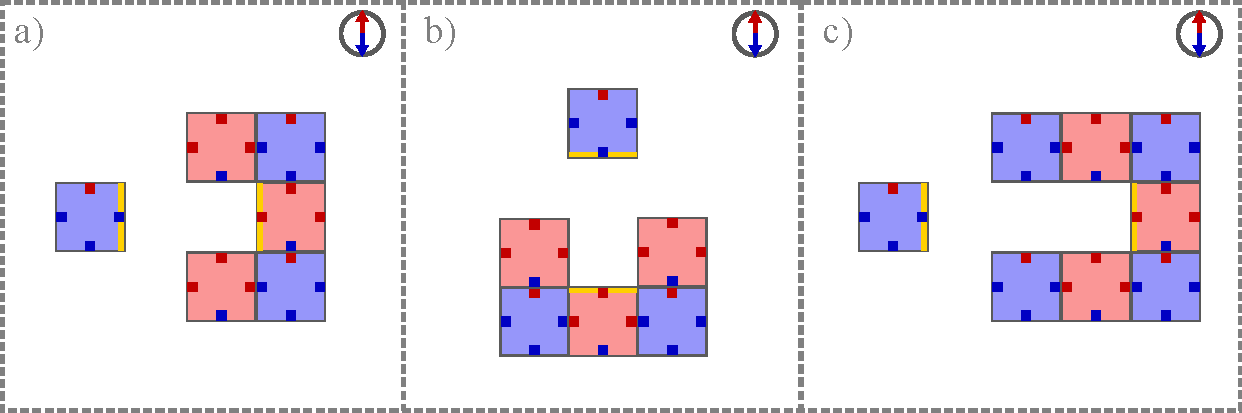
\includegraphics[width=0.80\textwidth]{figures/holes.pdf}
	\caption{Tree different examples for connecting polyominoes into holes. a) and b) show one-cube-deep holes (a) east-west and b) north-south). c) illustrates a two-cube-deep east-west hole. The edges to be connected are marked yellow.}
	\label{fig:holes}
\end{figure}

\paragraph{Connecting In Holes:}

Connecting two polyominoes where one of the connection-faces is located inside a hole, is a difficult task in the continuous world.
We differentiate between east-west and north-south located holes.
Furthermore a hole can be of a certain depth measured in multiples of $2 r_C$.
\autoref{fig:holes} shows examples for different holes with different depths.

Connecting into a hole with a depth of more than one times $2 r_C$ is not possible.
For instance, when inserting the blue single cube into the polyomino in \autoref{fig:holes} c), the blue cube would connect with north and south faces of the polyomino before even reaching the full depth of the hole.
But even holes with depth $2 r_C$ are hard to handle.
Inserting into a hole can be done by pivot walking, this would only work for east-west holes, or by letting magnetic forces attract the connection-faces.
Relying on magnetic forces alone seem promising, since it would work for both hole types, but in reality not only the forces of the connection-faces are present.
All the forces between other magnets prevent an easy slide-in.
In our simulator the connection-face will be more attracted or repelled by faces outside the hole, then the once inside.
Pivot walking into east-west holes, even with small values for $\alpha$, has also a high failure rate because of other magnets.
We generally try to avoid local plans that are connecting polyominoes inside holes.  

\section{Aligning Cubes}
\label{sec:align}



\section{Walking And Waiting}
\label{sec:walk_wait}



\section{Plan And Plan-State}
\label{sec:plan}



\section{Local Planning Algorithm}
\label{sec:local_algo}